\section{Tutorials 5 (28 III 2019)}
\textbf{1.} \underline{Problem}\\
In: a parity game $G$ and a positional strategy of Eve $\sigma$\\
Out: is $\sigma$ winning?\\
$\sigma$ is winning $\leftrightarrow$ $\forall_{\pi} G(\sigma, \pi) \in \textsc{Parity}$\\
$\sigma\ :\ V \rightarrow V$\\

\noindent
\textbf{2.} In: a parity game $G$, and an initial position $v_I$.\\
Out: Is $v_I$ winning for Eve?\\
Solution in \textsc{NP}:
\begin{itemize}
	\item guess the positional strategy of Eve $\rightarrow \sigma_{p}$
	\item check if $\sigma_p$ is winning
\end{itemize}
Solution in \textsc{coNP} -- check for strategy for Adam.\\
The problem is (at least) in $\textsc{NP} \cap \textsc{coNP}$\\

\noindent
\textbf{3.}\\
Muller $C \subseteq \mathbb{N}, \mathcal{F} \subseteq 2^{C}$\\
$C^{\omega} \ni p = a_1a_2...a_n...$ if $Inf(p) \in \mathcal{F}$ $\longleftarrow$ set of letters in $p$ that appears $\infty$-often\\
Parity -- $max(Inf(p))$ is even
\begin{itemize}
	\item[1)] Parity is Muller
	\item[2)] Muller is \underline{not} positionally determined
	\item[3)] Muller is not Parity
	\item[4)] Show that Muller is determined, what is the required memory?
	Show that if $G$ is a Muller game, then for every initial vertex $v_I$, one of the players has a winning strategy.
\end{itemize}
Solutions:
\begin{itemize}
	\item[1)] Parity game of index $(i, k)$ can be represented as a Muller game, where $\mathcal{F}$ consists
	of subsets of $\{i, i+1, ..., k\}$ with even maximum.
	\item[2)] Example below:\\
	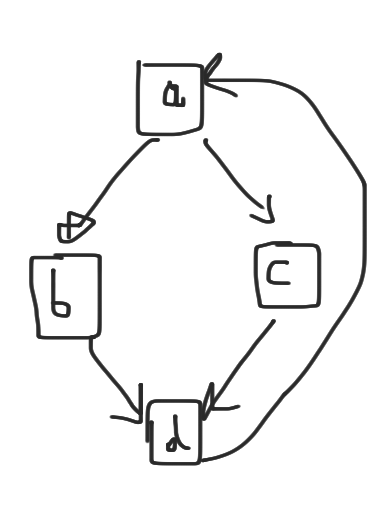
\includegraphics[scale=0.1]{content/graphics/game6}\\
	$\mathcal{F} = \{\{a, b, c, d\}\}$\\
	Every positional strategy removes either $b$ or $c$ and we require both.
	\item[3)] From (2)
	\item[4)] Idea: We will try to transform it to some Parity game, i.e.\\
	$G = \langle V, E, \lambda, v_I, \mathcal{F} \rangle \rightsquigarrow G^\prime = \langle V^\prime, E^\prime, \lambda^\prime, v_I^\prime, \textsc{Parity} \rangle$\\
	$E \subseteq V \times V$\\
	$\lambda\ :\ V \rightarrow C$\\
	s.t. $v_I$ is winning for Eve in $G \Leftrightarrow v_I'$ is winning for Eve in $G'$ (we need the same for Adam).
	In fact, we only need the implication to the left side.
\end{itemize}

\subsection*{LARs}
\textbf{LAR} (\textit{latest appearance record}) $w \in C \cup \{\natural\} (=\Gamma)$, every letter occurs at most once, $\natural$ occurs always.\\
$\textbf{up}\ :\ \text{LAR} \times \Gamma \rightarrow \Gamma$\\
$\textbf{up}(v_i \natural w_i, a) = \begin{cases}
	v_i \natural w_i a\ \ \ \ \ \ a \not\in v_i, a \not\in w_i\\
	[v_iw_i]_{a \mapsto \natural}a
\end{cases}$
